% Source: 2014 Shandong science q18 original PDF; schematic affine table projection.
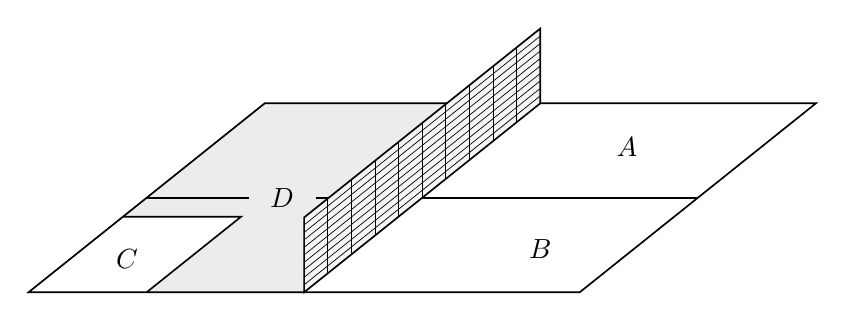
\begin{tikzpicture}[x=1cm,y=1cm,line width=.6pt,font=\normalsize]
\fill[gray!15] (0,0)--(3.5,0)--(6.5,2.4)--(3,2.4)--cycle;
\fill[white] (0,0)--(1.5,0)--(2.7,.96)--(1.2,.96)--cycle;
\draw (0,0)--(7,0)--(10,2.4)--(3,2.4)--cycle;
\draw (1.5,0)--(2.7,.96)--(1.2,.96);
\draw (1.5,1.2)--(2.8,1.2);
\draw (3.65,1.2)--(8.5,1.2);
\fill[gray!8] (3.5,0)--(6.5,2.4)--(6.5,3.35)--(3.5,.95)--cycle;
\foreach \t in {.1,.2,...,.9} {
\draw[line width=.25pt] ({3.5+3*\t},{2.4*\t})--({3.5+3*\t},{2.4*\t+.95});
\draw[line width=.25pt] (3.5,{.95*\t})--(6.5,{2.4+.95*\t});
}
\draw (3.5,0)--(6.5,2.4)--(6.5,3.35)--(3.5,.95)--cycle;
\node[inner sep=0pt] at (7.6,1.85) {$A$};
\node[inner sep=0pt] at (6.5,.55) {$B$};
\node[inner sep=0pt] at (1.25,.42) {$C$};
\node[inner sep=0pt] at (3.22,1.2) {$D$};
\end{tikzpicture}
